\subsection{Paquete 8: Asistente inteligente y orquestación de herramientas}

    El asistente virtual responde consultas en lenguaje natural apoyándose en Spring AI y en un servidor MCP (\emph{Model Context Protocol}). Permite filtrar habitaciones, consultar el estado de las tareas del hogar, resumir la mensajería entrante e inspeccionar colas de moderación. Para proteger los datos, el backend expide tickets efímeros con permisos de solo lectura antes de invocar las herramientas MCP. La figura \ref{fig:dcu_asistente_ia} expone los siete casos de uso del asistente (CU69 a CU75).

\begin{figure}[H]
    \centering
    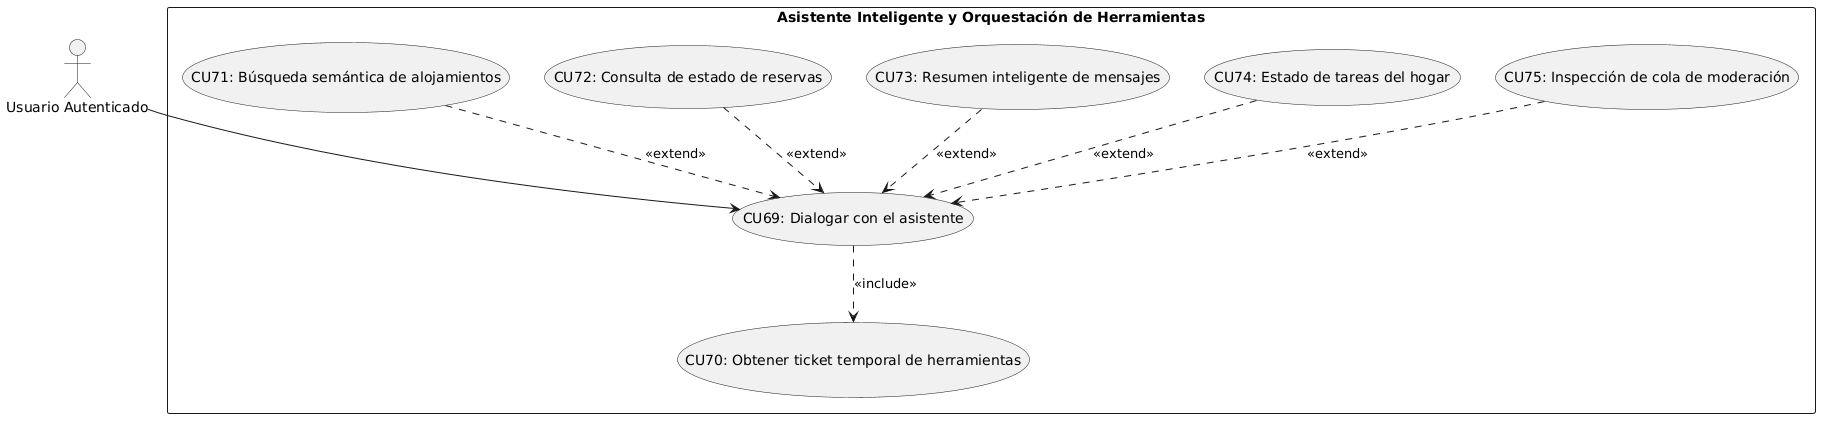
\includegraphics[width=0.82\textwidth]{AnalisisFuncional/img/dcu_asistente_ia.png}
    \caption{Diagrama de casos de uso de asistente inteligente y orquestación de herramientas}
    \label{fig:dcu_asistente_ia}
\end{figure}

    Las siguientes tablas detallan los casos de uso del agente inteligente (CU69 a CU75):

\begin{table}[H]
\centering
\begin{tabular}{|p{3.2cm}|p{11.3cm}|}
\hline
\textbf{Caso de Uso} & \textbf{CU69: Dialogar con el asistente en lenguaje natural} \\ \hline
\textbf{Actores} & Usuario Autenticado \\ \hline
\textbf{Descripción} & Mantiene una conversación interactiva con el agente inteligente mediante lenguaje natural \\ \hline
\textbf{Precondiciones} & Estar autenticado con una sesión activa en la aplicación \\ \hline
\textbf{Flujo básico} & 
1. El usuario abre el componente flotante de chat con el asistente e introduce una consulta. \newline
2. Se ejecuta de forma obligatoria la expedición de un ticket temporal de autorización para herramientas. \newline
3. El orquestador del backend procesa la petición evaluando si requiere invocar herramientas especializadas. \newline
4. El modelo genera la respuesta estructurada y la interfaz la visualiza mediante transmisión progresiva. \\ \hline
\end{tabular}
\caption{Especificación del caso de uso CU69}
\label{tab:cu69}
\end{table}

\begin{table}[H]
\centering
\begin{tabular}{|p{3.2cm}|p{11.3cm}|}
\hline
\textbf{Caso de Uso} & \textbf{CU70: Obtener ticket temporal de autenticación de herramientas} \\ \hline
\textbf{Actores} & Usuario Autenticado \\ \hline
\textbf{Descripción} & Emite una credencial temporal firmada para autorizar llamadas seguras al servidor de herramientas MCP \\ \hline
\textbf{Precondiciones} & Mantener un token de sesión JWT válido \\ \hline
\textbf{Flujo básico} & 
1. El subsistema de inteligencia artificial intercepta la interacción del usuario autenticado. \newline
2. El servicio emite un ticket criptográfico de corta duración vinculado al identificador del usuario. \newline
3. El backend traslada el ticket en las cabeceras de comunicación con el servidor MCP. \newline
4. El servidor MCP convalida la firma del ticket garantizando el aislamiento de privilegios. \\ \hline
\end{tabular}
\caption{Especificación del caso de uso CU70}
\label{tab:cu70}
\end{table}

\begin{table}[H]
\centering
\begin{tabular}{|p{3.2cm}|p{11.3cm}|}
\hline
\textbf{Caso de Uso} & \textbf{CU71: Herramienta: Búsqueda semántica por preferencias} \\ \hline
\textbf{Actores} & Usuario Autenticado \\ \hline
\textbf{Descripción} & Recupera anuncios considerando el estilo de vida, afinidad y descriptores cualitativos del usuario \\ \hline
\textbf{Precondiciones} & Que la consulta del usuario exprese requerimientos de convivencia o preferencias ambientales \\ \hline
\textbf{Flujo básico} & 
1. El modelo identifica la intención de localización cualitativa durante el diálogo con el asistente. \newline
2. El agente invoca de forma extendida la herramienta de búsqueda semántica con los criterios extraídos. \newline
3. El servidor MCP consulta el catálogo indexado y devuelve los alojamientos con mayor afinidad contextual. \newline
4. El asistente sintetiza la respuesta recomendando los inmuebles más adecuados en la conversación. \\ \hline
\end{tabular}
\caption{Especificación del caso de uso CU71}
\label{tab:cu71}
\end{table}

\begin{table}[H]
\centering
\begin{tabular}{|p{3.2cm}|p{11.3cm}|}
\hline
\textbf{Caso de Uso} & \textbf{CU72: Herramienta: Consulta de estado de reservas} \\ \hline
\textbf{Actores} & Usuario Autenticado \\ \hline
\textbf{Descripción} & Comprueba y resume el estado actual de las solicitudes de reserva emitidas o recibidas \\ \hline
\textbf{Precondiciones} & Que el usuario pregunte expresamente sobre la situación de sus estancias o reservas \\ \hline
\textbf{Flujo básico} & 
1. El modelo detecta una petición sobre el progreso de las reservas en curso. \newline
2. El agente ejecuta la llamada a la herramienta MCP transmitiendo el contexto de identidad del usuario. \newline
3. El servicio consulta la base de datos y compila las reservas pendientes, aceptadas o próximas a expirar. \newline
4. El asistente traslada un resumen conciso indicando las acciones pendientes que requiere cada solicitud. \\ \hline
\end{tabular}
\caption{Especificación del caso de uso CU72}
\label{tab:cu72}
\end{table}

\begin{table}[H]
\centering
\begin{tabular}{|p{3.2cm}|p{11.3cm}|}
\hline
\textbf{Caso de Uso} & \textbf{CU73: Herramienta: Resumen inteligente de mensajes} \\ \hline
\textbf{Actores} & Usuario Autenticado \\ \hline
\textbf{Descripción} & Sintetiza los temas clave y mensajes no leídos acumulados en la bandeja de entrada \\ \hline
\textbf{Precondiciones} & Disponer de mensajes recibidos en las conversaciones de la plataforma \\ \hline
\textbf{Flujo básico} & 
1. El usuario solicita al asistente conocer las novedades de sus conversaciones activas. \newline
2. El agente ejecuta condicionalmente la herramienta de agregación y análisis de mensajería. \newline
3. El servidor MCP recopila los hilos recientes omitiendo información confidencial no pertinente. \newline
4. El modelo estructura un extracto de las comunicaciones pendientes organizadas por remitente y urgencia. \\ \hline
\end{tabular}
\caption{Especificación del caso de uso CU73}
\label{tab:cu73}
\end{table}

\begin{table}[H]
\centering
\begin{tabular}{|p{3.2cm}|p{11.3cm}|}
\hline
\textbf{Caso de Uso} & \textbf{CU74: Herramienta: Estado de tareas del hogar} \\ \hline
\textbf{Actores} & Usuario Autenticado \\ \hline
\textbf{Descripción} & Proporciona una panorámica rápida sobre las tareas domésticas pendientes y las fechas límite en el piso \\ \hline
\textbf{Precondiciones} & Pertenecer activamente a un hogar constituido \\ \hline
\textbf{Flujo básico} & 
1. El usuario consulta mediante lenguaje natural por las labores domésticas que tiene pendientes. \newline
2. El asistente activa la herramienta MCP correspondiente consultando el módulo del hogar del usuario. \newline
3. El servicio devuelve las tareas asignadas para la semana, turnos rotativos y tareas susceptibles de rescate. \newline
4. El modelo expone el estado de las labores recordando los puntos asignados a cada una. \\ \hline
\end{tabular}
\caption{Especificación del caso de uso CU74}
\label{tab:cu74}
\end{table}

\begin{table}[H]
\centering
\begin{tabular}{|p{3.2cm}|p{11.3cm}|}
\hline
\textbf{Caso de Uso} & \textbf{CU75: Herramienta: Inspección de cola de moderación} \\ \hline
\textbf{Actores} & Usuario Autenticado \\ \hline
\textbf{Descripción} & Asiste en la revisión y diagnóstico rápido de reportes pendientes acumulados en la cola de incidencias \\ \hline
\textbf{Precondiciones} & Poseer el rol de administración del sistema (\emph{ADMIN}) \\ \hline
\textbf{Flujo básico} & 
1. Un administrador del sistema consulta al asistente sobre la carga actual de denuncias sin resolver. \newline
2. El agente comprueba los privilegios de administración del emisor y llama a la herramienta interna MCP. \newline
3. El servicio recopila las infracciones más graves y los usuarios reincidentes en la cola de moderación. \newline
4. El asistente sintetiza los expedientes prioritarios facilitando la toma de decisiones sancionadoras. \\ \hline
\end{tabular}
\caption{Especificación del caso de uso CU75}
\label{tab:cu75}
\end{table}